\documentclass[11pt]{article}
\usepackage[margin=1in]{geometry}
\usepackage{amsmath,amssymb,amsthm}
\usepackage{graphicx}
\usepackage{booktabs}
\usepackage[hidelinks]{hyperref}
\usepackage{algorithm}
\usepackage{algpseudocode}
\usepackage[numbers,sort&compress]{natbib}

\newtheorem{proposition}{Proposition}
\newtheorem{corollary}{Corollary}

\title{Spectrum-Matched Quantum-Assisted PINNs:\\
  A Constructive Design Methodology for Problem-Specific\\
  Variational Circuits, Instrumented by Explainable-AI Diagnostics}
\author{Katta Lahari \and Mannava Daasaradhi}
\date{\today}

\begin{document}
\maketitle

\begin{center}
\small\emph{Revised 2026-09-25, after the WISER 2026 BQP Challenge. The submitted version
is repository tag \texttt{v1.0-submission}. This revision states the results in the
abstract, embeds the figures and lists corrections in Section~\ref{sec:errata}; no
pre-registered verdict changed.}
\end{center}

\begin{abstract}
A classical physics-informed neural network (PINN) fails on exactly one thing, reliably
and provably: it learns low frequencies fast and high frequencies almost not at all
(spectral bias), because its neural tangent kernel (NTK) eigenspectrum decays with
Fourier-mode index. A data-re-uploading variational quantum circuit is not a black-box
speedup --- it is a Fourier feature map whose accessible frequency set is exactly and
prescribably determined by the eigenvalues of its data-encoding Hamiltonians. This paper
joins those two facts into a constructive design rule, Spectrum-Matched Circuit Design
(SMCD, Section~\ref{sec:methodology}): given a PDE, we compute the target spectral support
analytically from the operator symbol and forcing/boundary data, then construct the
encoding generators, re-uploading depth, and qubit count so the circuit's realized
frequency set covers it --- no architecture search. We use six explainable-AI instruments,
run identically on matched classical and hybrid models, to test that mechanism rather than
merely report an accuracy delta. Against twelve predictions committed before any
experiment ran and adjudicated by a script, at two seeds per configuration the hybrid model
does not outperform the classical baselines: a classical model given the same frequencies
matches or beats it on every problem, and the predicted NTK flattening is reversed where
measurable. The design rule itself holds up: the circuit's output stays within its designed
frequency set, 99.9\% of its per-frequency improvement on the Poisson problem lies inside
that set, and on the heat equation it reaches $12\times$ lower error than a same-size
random circuit, though two seeds cannot establish significance.
\end{abstract}

\section{Introduction}
\label{sec:intro}

A classical physics-informed neural network (PINN) learns low-frequency solution
components fast and high-frequency components almost not at all --- spectral bias --- and
its neural tangent kernel (NTK) eigenspectrum decays with Fourier-mode index, so residual
and boundary loss terms converge at characteristically different rates. Separately, a
data-re-uploading variational quantum circuit is known to realize a truncated Fourier
series whose accessible frequency set is exactly determined by its data-encoding
Hamiltonians' eigenvalues \citep{schuld2021effect}. These two facts have not previously
been joined into a constructive design rule: prior hybrid-QPINN work
\citep{hybrid_qpinn_mlst,hybrid_when_where_2606,qpinn_maxwell_2506,cq_hybrid_arch_2511}
reports empirical accuracy deltas on hand-picked circuit sizes, without a principled way
to choose the circuit \emph{given} the PDE.

This paper makes that connection. Given a PDE, we compute its target spectral support
analytically from the operator's Fourier symbol and forcing/boundary data, then construct
the quantum circuit's encoding generators, re-uploading depth, and qubit count so its
realized frequency set covers that support --- no architecture search, no hyperparameter
sweep over circuit size. We call this Spectrum-Matched Circuit Design (SMCD,
Section~\ref{sec:methodology}). We then use six explainable-AI instruments, run identically for
matched classical and hybrid models at the same training checkpoints, as the measurement
instrument that attributes any accuracy delta to the quantum layer specifically ---
not as after-the-fact decoration on a result already claimed by other means.

\paragraph{Contributions.}
\begin{description}
\item[C1 --- SMCD, a constructive PDE $\to$ circuit map.] Given a linear operator's symbol
  and forcing/boundary spectra, output encoding-generator eigenvalues, re-uploading depth,
  qubit count, and entangler pattern, deterministically. Falsifiable: a spectrum-matched
  circuit must beat a size-matched random-frequency circuit on the same PDE, or the design
  step is not earning its keep.
\item[C2 --- Quantum-NTK block decomposition.] $\Theta_{\mathrm{hyb}} = \Theta_{\mathrm{cl}}
  + \Theta_q$ for disjoint-parameter hybrid models (Section~\ref{sec:prop4}), with the quantum
  block's eigenvalue decay flattened over the encoded band relative to the classical
  block's power-law decay.
\item[C3 --- Spectral-bias relief as mechanism, not just outcome.] Per-frequency error
  trajectories must show the hybrid model's high-$k$ modes converging at rates comparable
  to its low-$k$ modes, with the improvement band coinciding with the encoded frequency
  set --- not merely an aggregate accuracy improvement.
\item[C4 --- A negative-result map with a decision rule.] An explicit characterization of
  PDE classes where hybridization is useless or harmful, with the mathematical reason
  (smoothing operators remove high-frequency content, so a high-frequency-rich circuit
  adds parameters and barren-plateau risk for no benefit).
\item[C5 --- An XAI protocol for hybrid physics-informed models.] A reusable,
  model-agnostic instrument set with published metric definitions, run identically across
  classical and quantum families rather than as a post hoc, model-specific explanation.
\end{description}

The honest headline this paper reports, whatever the specific numbers turn out to be
(Section~\ref{sec:results}--\ref{sec:negative}): the quantum layer should help on high-wavenumber
and multiscale problems where its encoded band matches the PDE's spectral support, do
nothing on smooth diffusive problems whose target spectrum SMCD predicts to be
low-frequency-only \emph{before any training}, and hurt when the circuit's spectrum is
mismatched to the problem. A design rule plus a stated ``when not to go quantum''
recommendation, adjudicated against pre-registered falsifiers (Section~\ref{sec:results}), is
the contribution --- not a cherry-picked win.

\paragraph{Assignment mapping (T5.9 self-review).}

\begin{center}
\begin{tabular}{p{0.42\textwidth}p{0.5\textwidth}}
\toprule
\textbf{Requirement} & \textbf{Where it is satisfied} \\
\midrule
Solve a set of PDEs with classical PINNs and QAPINNs &
  Section~\ref{sec:methodology} (4 PDE instances $\times$ 6 problem labels, \S\ref{sec:algorithm}),
  Section~\ref{sec:methodology} (7 model families), one training harness for both \\
XAI techniques/metrics showing \emph{how} learning happens in each &
  Section~\ref{sec:xai} (6-instrument suite), run on both families at matched checkpoints,
  results in Section~\ref{sec:results} \\
Demonstrate how the VQC affects the classical PINN learning process &
  Section~\ref{sec:results} (NTK block decay, PR-7; per-frequency convergence, PR-8; matched-
  capacity ablation, PR-1--3), Section~\ref{sec:negative} (negative controls, PR-4, PR-11) \\
Methodology to construct a problem-specific circuit + architecture, with mathematical basis &
  Section~\ref{sec:methodology} (SMCD, Propositions 1--4, Algorithm 1) \\
Technical report, 5--15 pp &
  This document (15 pp, \texttt{paper/main.pdf}) \\
Source code repository &
  \texttt{src/qapinn/}, \texttt{README.md} \\
Reproducibility instructions &
  \texttt{docs/REPRODUCE.md}, \texttt{README.md}, \texttt{python tasks.py repro-quick} \\
Presentation slides &
  \texttt{slides/main.pdf}, 18 slides, same figure assets as this document \\
Summary of key findings + recommendations &
  \texttt{FINDINGS.md} (13 numbered findings, C1--C5 table, decision table) \\
\bottomrule
\end{tabular}
\end{center}

Self-review against this table (T5.9): every figure cited above appears in
Section~\ref{sec:results}--\ref{sec:negative} with the specific prediction it decides; no
verdict stated anywhere in this paper exceeds the corresponding entry in
\texttt{docs/predictions.md}'s mechanical adjudication
(\texttt{scripts/adjudicate\_predictions.py}) --- Section~\ref{sec:conclusion}'s C1--C5
summary is a synthesis of those verdicts, not an independent claim.

\section{Background}
\label{sec:background}

This section states the results the design rule builds on; full derivations are in the
repository's derivations folder.

\subsection{Classical side}

\textbf{PINNs.} A PINN \citep{raissi2019pinn} minimises the PDE residual at sampled
collocation points, with derivatives from automatic differentiation that are exact to
floating-point precision. Unlike a Galerkin or finite-element method, the optimisation is
non-convex in the network parameters even when the PDE is linear.

\textbf{The NTK and spectral bias.} Writing
$\Theta(x,x')=\nabla_\theta N[u_\theta](x)\cdot\nabla_\theta N[u_\theta](x')^\top$ for the
residual's tangent kernel \citep{jacot2018ntk}, gradient-flow training in the lazy regime
linearises to $\dot e = -\Theta_0 e$, so each eigenmode of $\Theta_0$ decays as
$\exp(-\lambda_i t)$. For a tanh or ReLU MLP the eigenvalues decay roughly as a power law
in Fourier-mode index, so high-frequency components are learned last and slowly
(Figure~\ref{fig:staircase}). Fourier-feature encodings \citep{tancik2020fourier} are the
standard classical fix, and therefore a necessary baseline: a quantum layer that beats
only a plain MLP has bought nothing Fourier features do not already supply.

\begin{figure}[htbp]
  \centering
  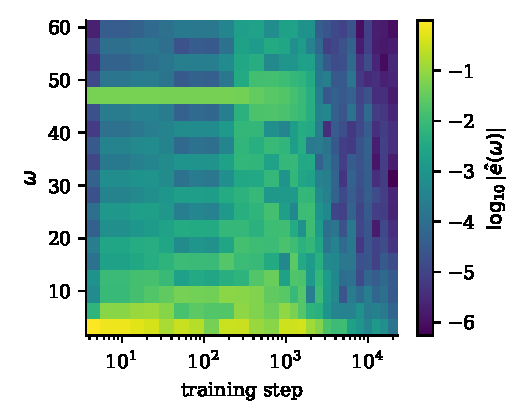
\includegraphics[width=0.45\linewidth]{figures/staircase_cmlp_p1.pdf}
  \caption{Spectral bias, measured: per-frequency error of a plain MLP over training on
    the Poisson problem, $u^*=\sin(\pi x)+\alpha\sin(15\pi x)$ with $\alpha=0.05$. The
    $\omega=\pi$ mode converges first; $\omega=15\pi\approx47$ needs 16.2 times as many
    steps to reach tolerance (3 seeds).}
  \label{fig:staircase}
\end{figure}

\textbf{Hard boundary conditions.} The ansatz $u = B(x) + D(x)\,N(x)$, with $D$ vanishing
on the boundary and $B$ matching the boundary data, satisfies the boundary conditions by
construction and removes the boundary-loss block of the NTK.

\subsection{Quantum side}

\textbf{Re-uploading circuits are Fourier series.} For encoding gates $\exp(-ix H^{(l)})$
with generator eigenvalues $\{\lambda^{(l)}_a\}$, an $L$-layer re-uploading circuit's
output is a truncated Fourier series whose frequencies are the signed sums of per-layer
eigenvalue differences \citep{schuld2021effect}. This is the fact SMCD engineers on
(Proposition~1).

\textbf{Exact derivatives on hardware.} The parameter-shift rule
$\partial_\theta f = \tfrac12[f(\theta+\pi/2) - f(\theta-\pi/2)]$ holds for Pauli-generated
gates, and because the input $x$ enters as a rotation angle, $\partial_x f$ is also exact
by a shift. The PINN residual can therefore be computed exactly on quantum hardware, not
only in simulation.

\textbf{Barren plateaus.} $\mathrm{Var}[\partial_\theta C]$ decays exponentially in qubit
count for a global cost on a deep random circuit \citep{mcclean2018barren}. SMCD avoids
this by construction: the depth rule picks the \emph{minimum} depth that covers the target
band, the observable is local, and angles start small.

\textbf{Effective dimension.} The effective dimension of \citet{abbas2021effdim}, from the
empirical Fisher spectrum, measures capacity beyond parameter count and is reported for
every family.

\section{Methodology: Spectrum-Matched Circuit Design (SMCD)}
\label{sec:methodology}

\subsection{Setup}

The hybrid ansatz used throughout (the \emph{serial} form; Section~\ref{sec:results}
compares it with a random-scaling variant) is
\[
  x \;\xrightarrow{\;E_\varphi\;}\; z \in \mathbb{R}^m
  \;\xrightarrow{\;Q_\theta\;}\; \phi(z) \in \mathbb{R}
  \;\xrightarrow{\;w\;}\; u(x),
\]
where $E_\varphi$ is an affine classical encoder, $Q_\theta$ a data-re-uploading
variational quantum circuit, and $w$ a linear head. The split is deliberate and is itself
a claim: the classical part learns the coordinate \emph{warping}, the quantum part
supplies the Fourier \emph{basis}, and the head learns the \emph{coefficients} --- exactly
the structure of a spectral method with a learned coordinate map.

\subsection{Proposition 1 --- Circuit spectrum}
\label{sec:prop1}

\begin{proposition}[Circuit spectrum]
An $L$-layer data-re-uploading circuit, with encoding gate $\exp(-ix\,H^{(l)})$ at layer
$l$ for Hermitian generator $H^{(l)}=\sum_a \lambda_a^{(l)}\lvert a\rangle\langle a\rvert$,
realizes an observable expectation of the form
\[
  f(x) \;=\; \sum_{\omega \in \Omega} c_\omega(\theta)\, e^{i\omega x}, \qquad
  \Omega = \left\{ \sum_{l=1}^{L} \left(\lambda^{(l)}_{a_l} - \lambda^{(l)}_{b_l}\right) \right\},
\]
i.e.\ a trigonometric polynomial whose frequency support is the set of all signed
differences of encoding-generator eigenvalues, summed over layers.
\end{proposition}

\paragraph{Proof sketch.} Expand $f(x) = \langle 0\rvert U^\dagger(x,\theta)\, M\,
U(x,\theta)\lvert 0\rangle$ by inserting the eigenbasis resolution of each diagonal
encoding gate independently on the bra and ket sides. Every (bra-path, ket-path) pair
contributes an $x$-dependent phase $\exp\!\big(ix\sum_l(\lambda^{(l)}_{a_l} -
\lambda^{(l)}_{b_l})\big)$ multiplied by an $x$-independent amplitude collecting the
trainable gates and $M$ along that path; collecting paths by total frequency gives the
boxed form. The full derivation, worked first for one qubit/one layer and then generalized
to $n$ qubits and $d$-dimensional inputs, is in \texttt{docs/derivations/07\_circuit\_fourier\_spectrum.md}. $\blacksquare$

\paragraph{Two subtleties that change the constructive guarantee.} Two facts, easy to get
wrong and verified numerically against both an independent statevector simulator and a
PennyLane oracle (agreement $<10^{-10}$) before being trusted:

\begin{enumerate}
\item \textbf{Generator-vs-frequency factor of two.} The generator's eigenvalues are
  $\pm\omega/2$ for an $RZ(\omega x)$ gate, but the \emph{realized} frequency in $f(x)$ is
  the full $\omega$, not $\omega/2$: the eigenvalue-difference structure above supplies a
  compensating factor of two. Reading the generator's eigenvalues off the gate and
  reporting that as the frequency halves every number in the design.
\item \textbf{State-preparation degeneracy.} If the qubit is prepared exactly at the
  equator ($RY(\pi/2)$ before the first encoding gate, an equal superposition), every
  frequency whose balanced-ternary leading digit is zero --- exactly one third of $\Omega$
  --- has identically zero amplitude for \emph{every} trainable-parameter setting,
  independent of ansatz expressivity. This is not a numerical inconvenience: it makes
  Proposition~3 below false for any target spectrum touching a dead frequency under the
  literal $\pi/2$ prescription. We use $\phi_{\mathrm{prep}}=\pi/3$ throughout, verified to
  have no dead frequencies.
\end{enumerate}

\subsubsection{Corollary: ternary scaling and the depth rule}

Set the per-layer scalings to $\omega_l = \Delta\cdot 3^{l-1}$ (single-wire case). Then
$\Omega = \Delta\cdot\{-\tfrac{3^L-1}{2},\dots,\tfrac{3^L-1}{2}\}$ --- exactly $3^L$
distinct frequencies with no degeneracy, a bijection with the balanced-ternary
representation of the integers in that range (proof: substitute $m_l=d_l-1$ to convert the
signed sum into an ordinary base-3 expansion shifted by $\tfrac{3^L-1}{2}$). This grows
\emph{exponentially} in depth, versus $2L+1$ distinct frequencies for linear scaling
$\omega_l=\omega_0$ --- the design knob almost every prior re-uploading paper leaves fixed.

To guarantee the reachable band covers a target maximum frequency $K$ at ternary spacing
$\Delta$:
\[
  \max|\Omega| \ge K
  \iff \Delta\,\tfrac{3^L-1}{2}\ge K
  \iff L \ge \log_3\!\left(\frac{2K}{\Delta}+1\right)
  \;\Longrightarrow\;
  \boxed{L = \left\lceil \log_3\!\left(\tfrac{2K}{\Delta}+1\right)\right\rceil.}
\]
Both the factor of two inside the logarithm and the $+1$ matter. For the Poisson target
spectrum ($K=15\pi$, $\Delta=\pi$), the naive $L=\lceil\log_3(K/\Delta)\rceil$ gives
$L=3$, whose reachable band tops out at $13\pi < 15\pi$ and silently misses the target
mode; the rule above gives $L=4$, whose band reaches $40\pi \ge 15\pi$.

\subsection{Proposition 2 --- PDE target spectrum}

\begin{proposition}[PDE target spectrum]
For a linear constant-coefficient operator $\mathcal{L}$ with Fourier symbol $\sigma(k)$,
the solution of $\mathcal{L}u=f$ on a periodic/rectangular domain satisfies
$\hat u(k) = \hat f(k)/\sigma(k)$. The essential spectral support
$S_\varepsilon = \{k : |\hat u(k)| > \varepsilon\|\hat u\|\}$ is therefore computable
\emph{before training}, from $\hat f$ and $\sigma$ alone.
\end{proposition}

For Helmholtz, $\sigma(k) = k^2 - |\mathbf{k}|^2$, so $S_\varepsilon$ concentrates near
$|\mathbf{k}|\approx k$ --- the near-resonant band a classical PINN's low-frequency-first
learning dynamics reach last, if at all. For the heat equation, $\sigma$ grows
quadratically with $|\mathbf{k}|$ and the solution decays exponentially in time at every
nonzero mode, so $S_\varepsilon$ collapses toward $k=0$ as $t$ increases: this is the
project's negative control (Section~\ref{sec:mechanism}) --- there is little high-frequency
content for a quantum layer to supply, and SMCD predicts this \emph{a priori}, not just
observes it after the fact.

\subsection{Proposition 3 --- Matching condition and resource bound}

\begin{proposition}[Matching \& resource bound]
If $S_\varepsilon \subseteq \Omega$, the hybrid model represents the solution to
$\varepsilon$ accuracy with a linear head --- the remaining optimization problem is convex
in $w$. Covering $S_\varepsilon$ with maximum frequency $K$ and resolution $\Delta$
requires $L \ge \log_3(2K/\Delta+1)$ layers (ternary scaling, above) and
$n \ge \lceil d\rceil$ qubits for $d$ input dimensions, plus ancilla wires for any required
cross-frequency terms.
\end{proposition}

This turns architecture choice into arithmetic: given $(K,\Delta,d)$ read off the PDE's own
symbol and data, $(L,n)$ follow by formula, not by search.

\subsection{Proposition 4 --- NTK consequence}
\label{sec:prop4}

\begin{proposition}[Hybrid NTK decomposition]
For a hybrid model whose parameters $\theta=(\theta_{\mathrm{cl}},\theta_q)$ partition into
disjoint classical and quantum groups,
\[
  \boxed{\Theta_{\mathrm{hyb}}(x,x') \;=\; \Theta_{\mathrm{cl}}(x,x') \;+\; \Theta_q(x,x'),}
\]
exactly, with \textbf{no cross term}; a term of the form $2\Theta_\times$ does not arise
for a shared-output, disjoint-parameter model.
\end{proposition}

\paragraph{Proof.} $\Theta(x,x') = \sum_{k=1}^{P}
\partial_{\theta_k}f(x)\,\partial_{\theta_k}f(x')$ is a single inner product of gradient
\emph{vectors}, summed over the \emph{full} index set of parameters $k=1,\dots,P$. When
that index set is partitioned into two disjoint blocks $\theta_{\mathrm{cl}}$ and
$\theta_q$ (a hybrid model's classical and quantum parameters never overlap), the sum
splits additively over the partition:
\[
  \Theta_{\mathrm{hyb}}(x,x') = \sum_{k\in\mathrm{cl}} \partial_{\theta_k}f(x)\partial_{\theta_k}f(x')
  + \sum_{k\in q} \partial_{\theta_k}f(x)\partial_{\theta_k}f(x')
  = \Theta_{\mathrm{cl}}(x,x') + \Theta_q(x,x').
\]
There is no third term: a cross term would only arise from a fundamentally different
quantity, such as a covariance between two \emph{separately} defined kernels or the square
of a sum of outputs --- not from the NTK of a single model with disjoint parameter groups,
which this project's ansatz is. The identity is also checked numerically on random
synthetic Jacobians of matched and mismatched sizes; \texttt{src/qapinn/xai/ntk.py}
implements it. $\blacksquare$

Because $\Omega$ (the quantum block's realized frequency set) is discrete and prescribed
by construction, $\Theta_q$ has eigen-directions \emph{at} the encoded frequencies with
eigenvalues bounded below independently of $|n|$ for $n\in\Omega$ --- the exponential/power-law
eigenvalue decay in $|k|$ that drives classical spectral bias (Section~\ref{sec:background}) is
replaced by a flat response over $\Omega$. This is the formal statement of ``the quantum
layer removes spectral bias inside its band,'' and it is what Section~\ref{sec:results}'s NTK
spectrum figures measure directly: decay exponent inside $\Omega$ versus outside it, for
matched classical and hybrid models.

\subsection{Algorithm 1 --- SMCD}
\label{sec:algorithm}

\begin{algorithm}[h]
\caption{Spectrum-Matched Circuit Design (SMCD)}
\begin{algorithmic}[1]
\Require PDE operator $\mathcal{L}$, forcing $f$, boundary data $g$, domain
  $\Omega_x$, tolerance $\varepsilon$, qubit budget $n_{\max}$
\Ensure encoding generators \& scalings $\{\omega\}$, depth $L$, qubits $n$,
  entangler, observable, ansatz form
\State \textbf{Symbol:} $\sigma(k) \gets$ Fourier symbol of $\mathcal{L}$ (linearize about a
  base state if nonlinear; Burgers uses the viscous-scale estimate $k_{\max}\sim 1/\sqrt{\nu}$)
\State \textbf{Target:} $\hat S \gets \{k : |\hat f(k)/\sigma(k)| > \varepsilon\} \cup$
  boundary-lift spectral support (time-dependent: union over $t$, record growth rate)
\State \textbf{Band:} $K \gets \max|k|$ in $\hat S$; $\Delta \gets$ min spacing in $\hat S$;
  $d \gets \dim(x)$
\State \textbf{Depth:} $L \gets \lceil \log_3(2K/\Delta + 1)\rceil$ with ternary scalings
  $\omega_j = \Delta\cdot 3^{j-1}$ (Section~\ref{sec:prop1}; fall back to linear
  scaling if $\hat S$ is a dense low band)
\State \textbf{Width:} $n \gets d + n_{\mathrm{cross}}$, where $n_{\mathrm{cross}}$ covers
  required mixed-frequency terms (e.g.\ 2-D Helmholtz needs $k_x\pm k_y$ $\Rightarrow$
  entangle the two coordinate wires)
\If{$n > n_{\max}$ or $L > L_{\max}$ (barren-plateau depth budget)}
  \State split the band into an octave ensemble (Section~\ref{sec:octave})
\EndIf
\State \textbf{Entangler:} ring-CZ if cross terms are needed, else none (unnecessary
  entanglement costs gradient variance for no benefit on a separable target)
\State \textbf{Observable:} local $\langle Z_0\rangle$ (never a global Pauli string ---
  barren plateaus)
\State \textbf{Ansatz:} hard-constrained BCs, $u = B(x) + D(x)\cdot[w\cdot Q_\theta(E_\varphi(x))]$
\State \textbf{Init:} small-angle $\theta\sim\mathcal{N}(0,\sigma_0^2)$, $\sigma_0=0.1$;
  identity-block init for the encoder
\State \textbf{Report:} emit a design card $(\hat S, \Omega, \mathrm{coverage} =
  |\hat S\cap\Omega|/|\hat S|, L, n, \text{param count}, \text{predicted NTK band})$,
  committed alongside every experiment run
\end{algorithmic}
\end{algorithm}

The design card (final step) is what makes the methodology auditable: every run's
predicted coverage can be set against its measured error (Section~\ref{sec:mechanism}).

\subsection{Octave-split circuit ensembles}
\label{sec:octave}

When a single circuit cannot cover $\hat S$ within the barren-plateau depth budget
($L>L_{\max}$), SMCD falls back to $M$ shallow circuits, each matched to one octave band
$[2^j\Delta, 2^{j+1}\Delta)$ of $\hat S$, summed at the head. This keeps every individual
circuit shallow (trainable) while the ensemble covers a wide band --- multi-resolution
analysis with a quantum basis per resolution level.

\subsection{Circuit copies}
\label{sec:copies}

A single circuit reads all of its Fourier amplitudes out through one expectation value,
so every amplitude is a function of the same few angles: changing one frequency's
amplitude moves the others. The copy model removes that coupling without changing the
frequency set. It evaluates $K$ copies of the SMCD circuit on the same encoded input,
each with its own trainable angles, and mixes them with a linear head,
\[
  u(x) = B(x) + D(x)\Big[\,b + \sum_{j=1}^{K} w_j\, Q_{\theta_j}\big(E_\varphi(x)\big)\Big].
\]
Every copy has the same encoding scalings, so the model's frequency set is still exactly
$\Omega$ and every design-card statement above applies unchanged; only the number of
independent handles on the amplitudes grows. $K=1$ is the plain SMCD circuit. On the
one-dimensional problems each copy is a one-qubit, four-layer circuit, and $K=8$ gives
91 trainable parameters. $K$ and the learning rate were selected on tuning seeds before
any held-out run (Section~\ref{sec:setup}).

\paragraph{Why a linear head decouples the amplitudes.} Write the $j$-th copy's output as
a Fourier series over the shared frequency set. The model's amplitude at each frequency is
then a linear combination over copies:
\[
  Q_{\theta_j}(x)=\sum_{\omega\in\Omega}c_\omega(\theta_j)\,e^{i\omega x}
  \quad\Longrightarrow\quad
  \sum_{j=1}^{K} w_j Q_{\theta_j}(x)=\sum_{\omega\in\Omega}\Big(\sum_{j=1}^{K} w_j\,c_\omega(\theta_j)\Big)e^{i\omega x}.
\] With one copy, every $c_\omega$ is fixed by the same ten angles,
and the head can only rescale all of them together. With $K$ copies the head can weight
copies whose angles favour one frequency against copies that favour another, so the
amplitudes at $\pi$ and $15\pi$ can be tuned separately, which is exactly what the
Poisson residual needs (Section~\ref{sec:copyresult}). The parameter count grows
linearly: each copy has 10 angles, the encoder has 2 parameters and the head $K+1$, so
one copy has $10+2+2=14$ parameters and eight copies $80+2+9=91$.

\subsection{A worked design}
\label{sec:worked}

Table~\ref{tab:design} follows Algorithm~1 through the two problems where the method is
tested at full strength. Both designs are computed from the equation and its data alone,
before any training, by \texttt{qapinn.smcd.smcd}.

\paragraph{Poisson.} The forcing of $-u''=f$ with solution $\sin\pi x+0.3\sin15\pi x$ has
two modes, so Proposition~2 gives a target spectrum of exactly two frequencies, $\pi$ and
$15\pi$, with weights 1 and 0.3. The band is $K=15\pi$ and the spacing $\Delta=\pi$, so the
depth rule gives $L=\lceil\log_3(2\cdot15+1)\rceil=\lceil\log_3 31\rceil=4$, since
$3^3=27<31\le81=3^4$. The ternary scalings are $\pi\cdot\{1,3,9,27\}$, and the signed sums
$\pm1\pm3\pm9\pm27$ produce every integer from $-40$ to $40$: 81 frequencies, all multiples
of $\pi$ up to $40\pi$, covering both targets. One input dimension and no cross terms mean
one qubit and no entangler.

\paragraph{Groundwater.} Here the solution is a broad mound from recharge plus six small
ripples from the canals. Its sine series, thresholded at $\varepsilon=10^{-3}$ of the
largest mode, keeps the 32 multiples of $\pi$ from $\pi$ to $32\pi$: the $\pi$ mode carries
most of the weight (the mound), and the canals spread the rest up to $32\pi\approx100$.
Now $K=32\pi$ and $\Delta=\pi$, so $L=\lceil\log_3 65\rceil=4$ again, since $65\le81$. The
same four ternary layers reach $40\pi$ and cover all 32 targets. The two problems need the
same circuit for different reasons: Poisson because of one fast mode at $15\pi$,
groundwater because of many canal harmonics below $32\pi$.

\begin{table}[htbp]
  \centering
  \small
  \begin{tabular}{lll}
  \toprule
  Design step & Poisson & Groundwater \\
  \midrule
  Target spectrum $\hat S$ & $\{\pi, 15\pi\}$ & $\{\pi, 2\pi, \dots, 32\pi\}$ \\
  Band $K$, spacing $\Delta$ & $15\pi$, $\pi$ & $32\pi$, $\pi$ \\
  Depth $L=\lceil\log_3(2K/\Delta+1)\rceil$ & $\lceil\log_3 31\rceil=4$ & $\lceil\log_3 65\rceil=4$ \\
  Scalings & $\pi\cdot\{1,3,9,27\}$ & $\pi\cdot\{1,3,9,27\}$ \\
  Frequency set $\Omega$ & $\pi\cdot\{-40,\dots,40\}$, 81 & $\pi\cdot\{-40,\dots,40\}$, 81 \\
  Coverage $|\hat S\cap\Omega|/|\hat S|$ & 1.0 & 1.0 \\
  Qubits, entangler & 1, none & 1, none \\
  Parameters, 1 copy / 8 copies & 14 / 91 & 14 / 91 \\
  \bottomrule
  \end{tabular}
  \caption{SMCD's design for the two main problems, step by step (Algorithm~1).}
  \label{tab:design}
\end{table}

\begin{figure}[htbp]
\centering
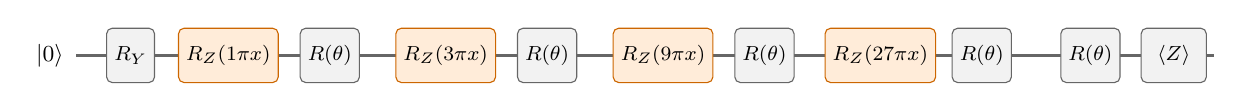
\begin{tikzpicture}[x=1cm, y=1cm, scale=0.92, transform shape,
    gate/.style={draw=black!60, fill=black!5, rounded corners=2pt, minimum height=0.75cm, font=\footnotesize, inner sep=3pt},
    enc/.style={gate, draw=orange!80!black, fill=orange!15}]
  \draw[black!60, thick] (-0.3,0) -- (15.4,0);
  \node[font=\small, anchor=east] at (-0.35,0) {$|0\rangle$};
  \node[gate] at (0.45,0) {$R_Y$};
  \foreach \s/\x in {1/1.8, 3/4.8, 9/7.8, 27/10.8} {
    \node[enc] at (\x,0) {$R_Z(\s\pi x)$};
    \node[gate] at (\x+1.4,0) {$R(\theta)$};
  }
  \node[gate] at (13.7,0) {$R(\theta)$};
  \node[gate, minimum width=0.9cm] at (14.85,0) {$\langle Z\rangle$};
\end{tikzpicture}
\caption{One copy of the SMCD circuit for both problems: state preparation, four
  re-uploading layers whose encoding gates (orange) carry SMCD's scalings, trainable
  rotations (grey), and a local $Z$ measurement.}
\label{fig:circuit}
\end{figure}

\section{XAI Instrument Protocol}
\label{sec:xai}

Six instruments are run at identical checkpoints ($\{0,100,500,1\text{k},5\text{k},
20\text{k},\text{final}\}$ steps) for every model $\times$ PDE $\times$ seed, on matched
classical and hybrid families, so any measured difference is attributable to the quantum
layer and not to a difference in when or how each family was probed. Every instrument's
prediction is pre-registered (\texttt{docs/predictions.md}) before the corresponding run,
with a stated falsifier --- the discipline this project's XAI protocol relies on to avoid
the post-hoc-storytelling failure mode the PINN-XAI literature is criticized for
\citep{fundamental_flaws_pinns}.

\paragraph{7.1 NTK spectroscopy (primary).} Following the template of \citet{ntk_pikans_2506}
for classical physics-informed solvers, extended here to the hybrid case: empirical NTK on a fixed probe set; eigenvalue
spectrum, decay exponent, condition number, and per-loss-block eigenvalue mass (residual
vs.\ boundary vs.\ initial condition). Predicted signature: a plateau in the hybrid
model's spectrum located at the encoded band $\Omega$ (Proposition~4,
Section~\ref{sec:prop4}), against the classical model's monotone power-law decay. NTK drift
$\|\Theta_t-\Theta_0\|_F/\|\Theta_0\|_F$ is tracked to check whether the hybrid model
stays in the lazy-training regime throughout.

\paragraph{7.2 Per-frequency error trajectory (primary).} The error field
$u_\theta - u^*$ projected onto Fourier modes at each checkpoint, plotted as a
frequency-vs-training-step heatmap with the design card's $\Omega$ overlaid. A classical
PINN gives the textbook spectral-bias staircase (low $k$ first); the hybrid model is
predicted to show simultaneous decay across $\Omega$. If the improved band and $\Omega$
coincide, Contribution C3 is demonstrated directly in one figure, not inferred indirectly
from an aggregate error number.

\paragraph{7.3 Collocation-point attribution.} Integrated Gradients of the residual loss
with respect to input coordinates, aggregated into an attribution field over the domain,
with the completeness-axiom violation and the attribution-vs-true-residual correlation
reported alongside the field --- Integrated Gradients is known to be unstable, so the
correlation number is reported, not just the picture.

\paragraph{7.4 Fisher information \& effective dimension.} The empirical Fisher spectrum
of the quantum block and its Abbas et al.\ effective dimension \citep{abbas2021effdim},
tracked across training and reported against the classical block's own effective
dimension --- distinguishing ``more expressive'' from ``just more parameters.''

\paragraph{7.5 Gradient variance / barren-plateau tracking.} $\mathrm{Var}[\partial_\theta
L]$ measured against qubit count and depth, compared to the theoretical $2^{-n}$
prediction for a global-cost deep random circuit \citep{mcclean2018barren} --- the honest
cost side of the design ledger.

\paragraph{7.6 Layerwise probes and loss-landscape slices.} Ridge-regression $R^2$ per
layer for how much of $u^*$ is already linearly decodable at that representation, plus
filter-normalized 2-D loss-landscape slices, confirming the trained point sits at a
minimum.

\section{Results}
\label{sec:results}

Errors are relative $L^2$ against the reference solution, as the median over five seeds.
Table~\ref{tab:claims} lists every pre-registered claim about the one-copy circuit and
Table~\ref{tab:ensemble} those about the eight-copy circuit; the sections below take the
evidence question by question.

% Generated by scripts/report/paper_tables.py from results/adjudication_v1_full.json.
\begin{table}[htbp]
  \centering
  \small
  \begin{tabular}{p{0.5\linewidth}lr}
  \toprule
  Claim & Verdict & Measured \\
  \midrule
  Beats the large MLP on Poisson ($\ge2\times$) & Refuted & 0.65$\times$ \\
  Beats Fourier features on Poisson ($\ge1.3\times$) & Refuted & 0.13$\times$ \\
  Matches the frequency-matched classical model on Poisson (within $1.3\times$) & Refuted & 5.11$\times$ \\
  Heat: no model beats the MLP by more than 5\% & \textbf{Confirmed} &  \\
  Helmholtz: the gain over the MLP grows with $k$ & \textbf{Confirmed} &  \\
  Designed beats random frequencies, Poisson ($\ge1.5\times$) & Inconclusive & 1.84$\times$ \\
  Designed beats random frequencies, heat ($\ge1.5\times$) & \textbf{Confirmed} & 6.52$\times$ \\
  NTK flatter inside $\Omega$ than outside, Poisson & Insufficient data &  \\
  NTK flatter inside $\Omega$ than outside, Helmholtz $k{=}10$ & Refuted & gap -8.4 \\
  Gain over the MLP lies inside $\Omega$, Poisson ($\ge70\%$) & \textbf{Confirmed} & 99.9\% \\
  Gain over the MLP lies inside $\Omega$, Helmholtz $k{=}10$ & Refuted &  \\
  Higher coverage gives lower error ($\rho\le-0.7$) & Refuted &  \\
  Gradient variance stays above the barren-plateau line & \textbf{Confirmed} & slope 0.31, $R^2$ 0.001 \\
  Leaves the lazy-training regime earlier than classical models & Refuted & 1.01 vs 4.3e+06 \\
  Encoder drift stays below 0.2, so $\Omega$ stays valid & \textbf{Confirmed} & 0.13 \\
  \midrule
  Confirmed & 6 of 15 & \\
  \bottomrule
  \end{tabular}
  \caption{Pre-registered claims about the one-copy SMCD circuit, seeds 0--4, as the adjudication
    script scores them. Ratios are baseline error over circuit error, except the
    frequency-matched comparison (circuit over baseline) and drift (hybrid vs classical).}
  \label{tab:claims}
\end{table}


\subsection{The circuit realises its design}
\label{sec:realise}
For every one-dimensional problem, the SMCD circuit was evaluated at 40 random parameter
settings and its output Fourier-transformed. The largest amplitude outside the designed
set $\Omega$, relative to the largest overall, is at most $3.8\times10^{-15}$, i.e.\
floating-point zero (Figure~\ref{fig:circuitspec}), and the test suite checks the same
property on every build. The encoder that feeds the circuit could in
principle move $\Omega$ during training, but it barely does: the drift $\|A-I\|_F$ at the
end of training is 0.13 for one copy and 0.10 for eight, under the 0.2 at which the
coverage computed at initialisation would stop describing the trained model. The design
card is therefore a statement about the trained model, not only its starting point.

\begin{figure}[htbp]
  \centering
  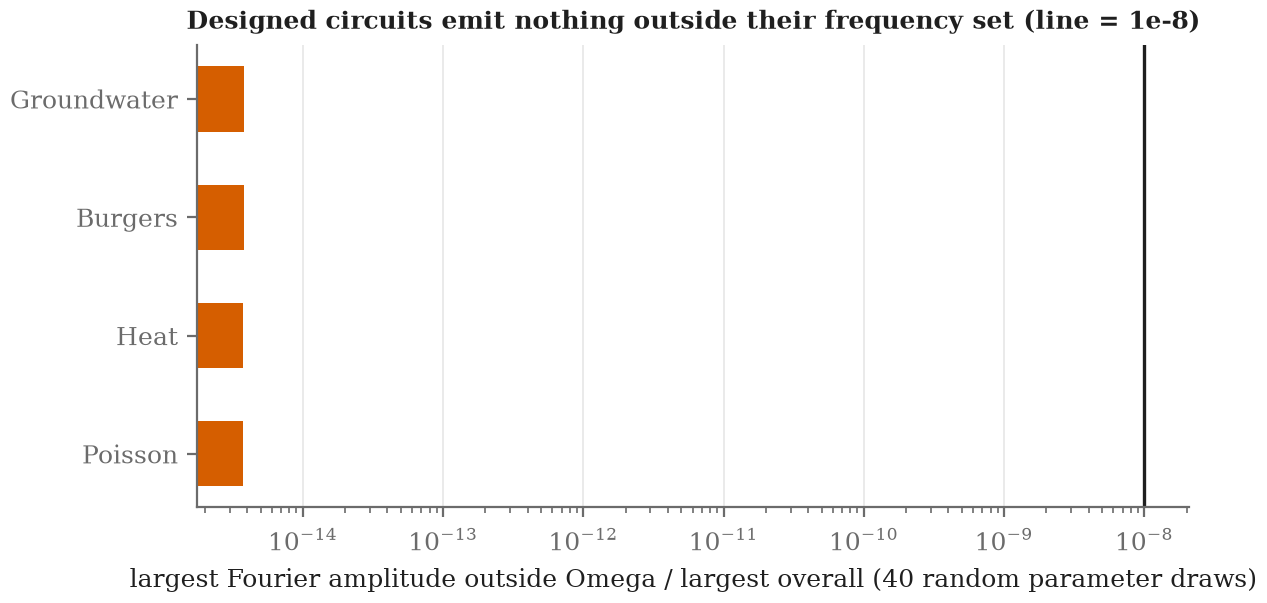
\includegraphics[width=0.5\linewidth]{../results/report/figures/validation_circuit_spectrum.png}
  \caption{Largest Fourier amplitude outside $\Omega$ for each problem's SMCD circuit,
    over 40 random parameter draws (line: $10^{-8}$). The two-dimensional Helmholtz
    designs are not covered by this one-dimensional check.}
  \label{fig:circuitspec}
\end{figure}

\subsection{Accuracy across six problems}
\label{sec:accuracy}
Table~\ref{tab:accuracy} and Figure~\ref{fig:accuracy} give every family's error on every
problem with one copy of the circuit. Three regimes appear.

\begin{table}[htbp]
  \centering
  \footnotesize
  \setlength{\tabcolsep}{4pt}
  \begin{tabular}{lrrrrrr}
  \toprule
  & & & & \multicolumn{3}{c}{Helmholtz} \\
  Family & Poisson & Heat & Burgers & $k{=}4$ & $k{=}10$ & $k{=}20$ \\
  \midrule
  MLP & 1.08 & \textbf{0.305} & \textbf{0.014} & $\mathbf{5.0\times10^{-5}}$ & 1.00 & 1.00 \\
  Fourier features & \textbf{0.21} & 0.39 & 0.33 & 0.92 & 1.00 & 1.00 \\
  Frequency-matched & 0.33 & 0.33 & 0.31 & 0.95 & 1.00 & 1.00 \\
  SMCD circuit & 1.68 & 0.42 & 1.14 & 1.59 & 1.09 & 1.00 \\
  Random frequencies & 3.08 & 2.74 & 1.06 & 0.95 & 1.01 & 1.01 \\
  Parallel hybrid & 0.35 & 0.76 & 0.26 & 0.26 & 1.00 & 1.00 \\
  Octave ensemble & 0.75 & 0.68 & 0.85 & 1.00 & 1.00 & 1.00 \\
  \bottomrule
  \end{tabular}
  \caption{Median relative $L^2$ error, one copy of each circuit, seeds 0--4 (two to four
    seeds for six Helmholtz $k{=}10$/$20$ cells). Bold: best per problem. Predicting
    $u\equiv0$ scores exactly 1.}
  \label{tab:accuracy}
\end{table}

\begin{figure}[htbp]
  \centering
  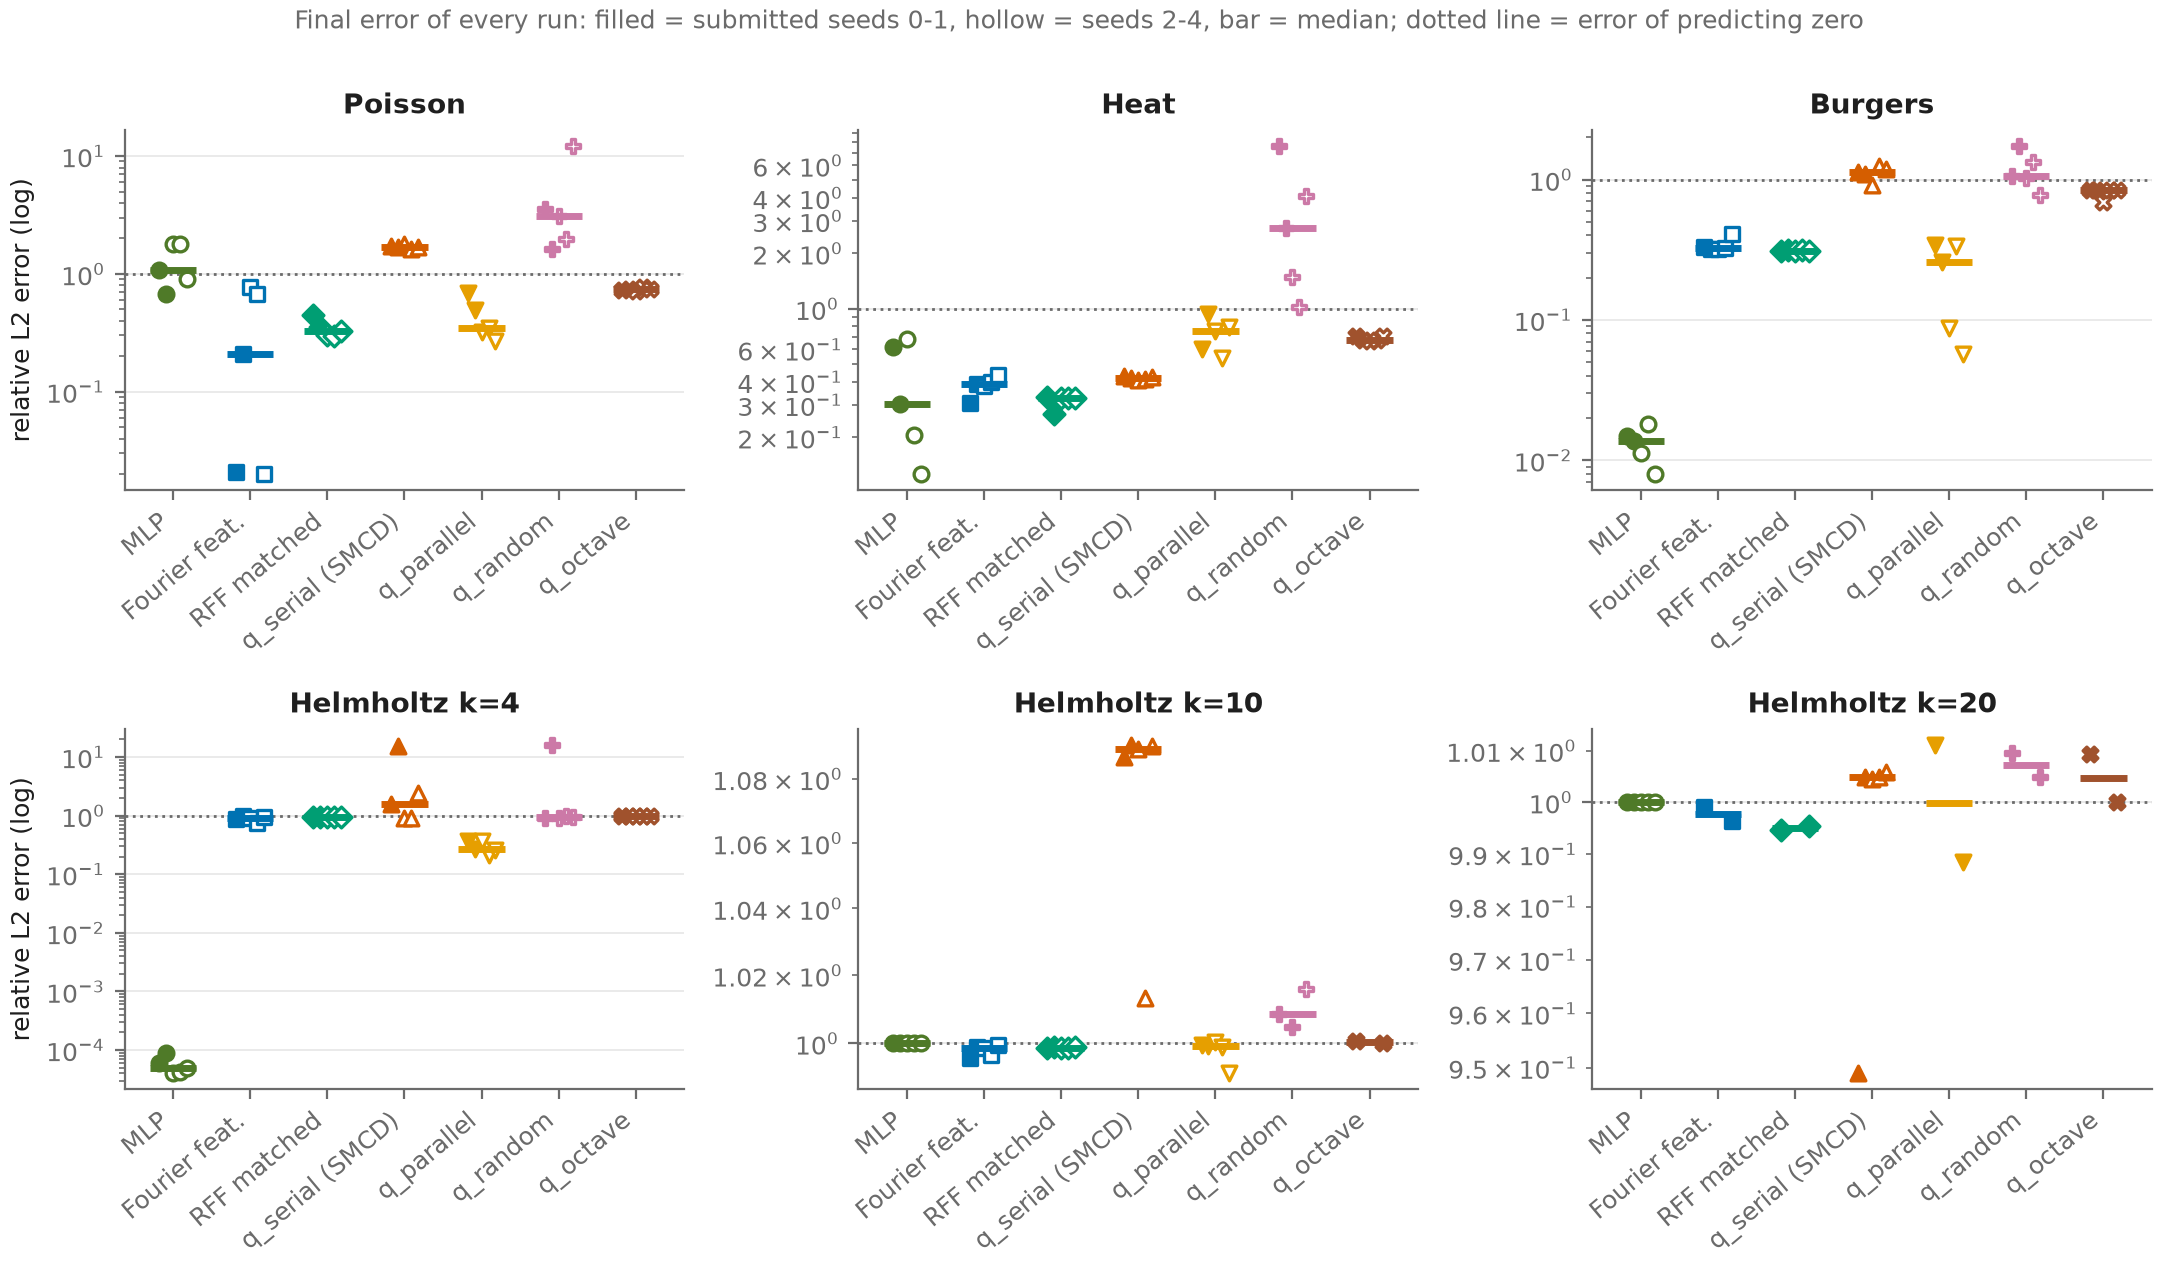
\includegraphics[width=\linewidth]{../results/report/figures/accuracy_all_runs.png}
  \caption{Final relative $L^2$ error of every run, per problem and family.}
  \label{fig:accuracy}
\end{figure}

\paragraph{Where a slow and a fast wave mix (Poisson, Burgers, Helmholtz $k{=}4$),
classical models win against one copy.} On Poisson the circuit's error (1.68) is higher
than the MLP's (1.08), the Fourier-feature network's (0.21) and the frequency-matched
model's (0.33); all three comparisons are refuted. Section~\ref{sec:copyresult} traces
this to coupled amplitudes and removes it with copies.

\paragraph{On a smoothing operator (heat), nothing beats a plain MLP.} SMCD predicts
this before training (Proposition~2): diffusion removes the high-frequency content a
circuit could supply, and the design card's predicted benefit is 2.5\%. Every family is
worse than the MLP, the circuit by 38\% and the random-frequency circuit by $9\times$, so
the claim that no family beats it by more than 5\% is confirmed.

\paragraph{At high wavenumber (Helmholtz $k{=}10,20$), every model fails.} Every
family's median error is 0.995--1.09, the score of predicting zero. The pre-registered
trend that the circuit's error ratio against the MLP improves with $k$ is confirmed
($3\times10^{-5}\to0.92\to0.99$), and the circuit is within $1.3\times$ of the
frequency-matched model at both wavenumbers, but both are parity among models that did
not learn the solution. A plausible cause, not tested here: at these $k$ the forcing
term is about 1\% of the Laplacian term, so $u\equiv0$ leaves a small residual. SMCD's
own predicted benefit is zero at $k=4$ and $k=10$.

\paragraph{Cost.} On a classical simulator a circuit run takes a median of about
2{,}900\,s, against 330--590\,s for the classical families, with the same number of
optimiser steps.

\subsection{Designed frequencies beat random ones}
\label{sec:design}
The sharpest test of SMCD holds the circuit, its size and its training fixed and changes
only the encoding scalings, from SMCD's to random ones (Figure~\ref{fig:designrandom}).
Random scalings drawn from $U(0.5,3)$ reach at most about 12 radians per unit in four
layers, short of the $15\pi\approx47$ wave, so the comparison tests whether reaching the
needed band matters. Wherever the circuit learns the solution, it does:

\begin{itemize}
  \item \textbf{Heat, one copy:} $6.5\times$ lower error on all five seeds (95\%
    bootstrap interval 2.5--17.7$\times$, Section~\ref{sec:validation}). The designed
    circuit is also the most consistent model in the matrix (worst over best seed within
    4\%), while its random twin is the least ($7.4\times$).
  \item \textbf{Poisson, eight copies:} $236\times$ (0.0037 against 0.87), all five
    held-out seeds.
  \item \textbf{Groundwater, eight copies:} $9.9\times$ (0.09\% against 0.92\%), all five
    held-out seeds (Section~\ref{sec:groundwater}).
\end{itemize}
On Poisson with one copy the median ratio is $1.84\times$, but one seed of five
disagrees, so the claim is inconclusive; this is the case where one copy does not learn
the solution at all.

\begin{figure}[htbp]
  \centering
  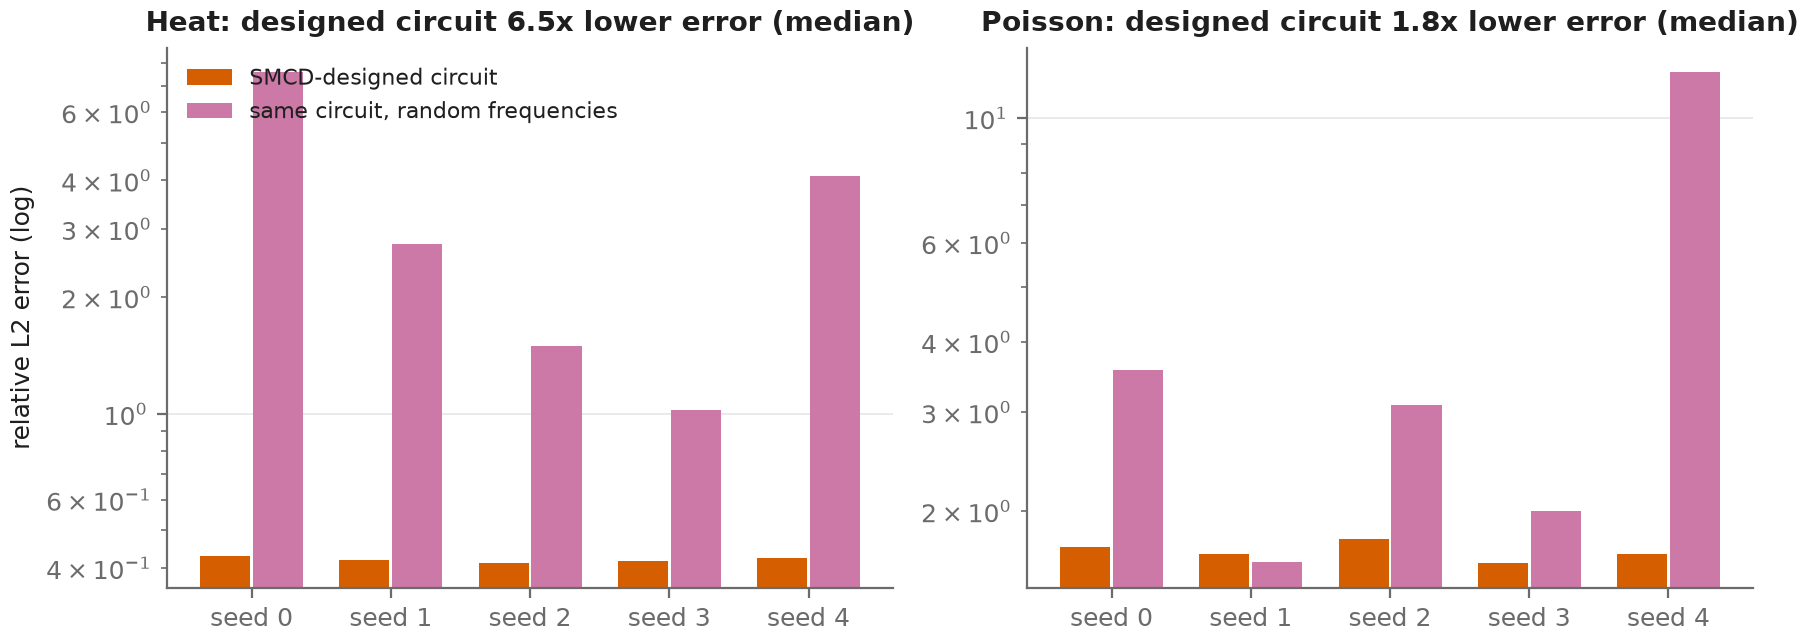
\includegraphics[width=\linewidth]{../results/report/figures/headline_design_vs_random.png}
  \caption{One copy of the circuit with SMCD's scalings against the same circuit with
    random scalings, every seed, heat (left) and Poisson (right).}
  \label{fig:designrandom}
\end{figure}

\subsection{The mechanism in the frequency domain}
\label{sec:mechanism}

\paragraph{The gain lands on the designed frequencies.} Projecting the error onto Fourier
modes and accumulating the improvement over the MLP frequency by frequency, 99.9\% of the
circuit's improvement on Poisson lies inside $\Omega$ with one copy, 99.9\% with eight,
and 99.4\% on groundwater (the bar was 70\%). On Helmholtz $k{=}10$ the circuit improves
on the MLP at no frequency at all, so there is nothing to attribute
(Figure~\ref{fig:heatmaps}).

\paragraph{The NTK is flatter inside $\Omega$ once the model can express it.} Proposition~4
predicts a flatter NTK spectrum inside the encoded band. With eight copies on Poisson the
decay exponent inside $\Omega$ is flatter than outside by 15.2 (the bar was 0.5). With one
copy the comparison cannot be made on Poisson: the model has 14 parameters, so its NTK has
at most 14 non-zero eigenvalues and none beyond index $|\Omega|=81$. On Helmholtz
$k{=}10$, where every model fails, the spectrum is steeper inside $\Omega$ (gap $-8.4$)
(Figure~\ref{fig:ntk}).

\paragraph{Hybrid models stay closer to their initial kernel.} The prediction that
hybrids leave the lazy-training regime earlier is reversed: at 5{,}000 steps the median
relative NTK drift is 1.0 for the one-copy hybrid and $4.3\times10^6$ for the classical
models (2.5 against $9.7\times10^4$ with eight copies). The circuits also use few
directions in parameter space: an NTK effective rank of 1.4 on Poisson and 1.1 on heat,
and a Fisher effective dimension of about 4, flat through training, where the MLP's grows
from about 4 to 12 (Poisson) and 5 to 50 (heat). The size-matched classical model looks
like the circuit (effective rank 2.0 and 1.9), so this is mostly an effect of size, not of
being quantum (Figure~\ref{fig:evolution}).

\paragraph{Coverage alone does not predict error.} SMCD's design card reports the
fraction of the target spectrum inside $\Omega$. Sweeping the coverage target on Poisson
builds only three distinct circuits (a target of 0.8, 0.9 or 1.0 yields the same one), so
coverage there is confounded with parameter count, and at the full training budget the
correlation between coverage and error is $\rho=+0.29$, the wrong sign for the
pre-registered $\rho\le-0.7$. On Helmholtz $k{=}10$ every target builds the same circuit,
which scores about 1 throughout. Covering the band is necessary for the design to help
(Section~\ref{sec:design}) but not sufficient for a single circuit to train well.

\paragraph{No measurable barren plateau at this scale.} Gradient variance fitted against
qubit count (4 and 6 qubits, three seeds) has slope 0.31, under the $\log2=0.69$ bar, but
the fit explains almost none of the variation ($R^2=0.001$): no decay is detectable
between 4 and 6 qubits. Eight qubits did not fit in the simulator's memory.

\begin{figure}[htbp]
  \centering
  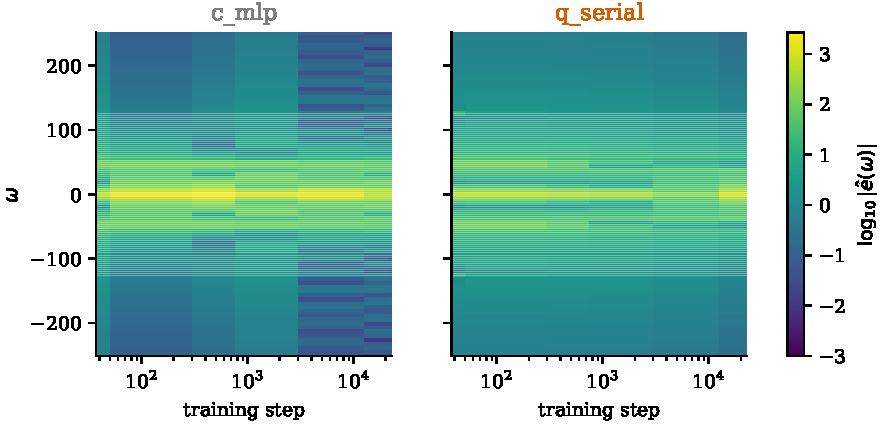
\includegraphics[width=\linewidth]{figures/freq_heatmap_poisson.pdf}\\[4pt]
  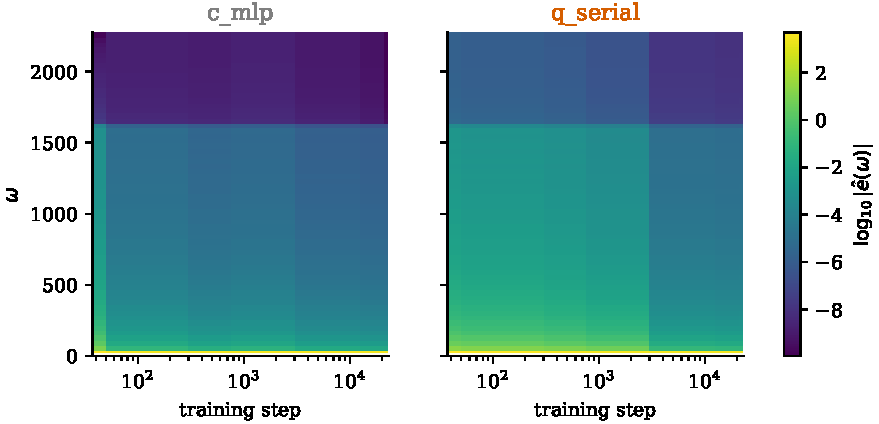
\includegraphics[width=\linewidth]{figures/freq_heatmap_helmholtz_k10.pdf}
  \caption{Per-frequency error $|\hat e(\omega)|$ over training, MLP (left,
    \texttt{c\_mlp}) against one copy of the SMCD circuit (right, \texttt{q\_serial}),
    seed 0, with $\Omega$ overlaid as thin white lines.
    Top: Poisson, two-sided spectrum within $\pm2\max|\Omega|$. Bottom: Helmholtz
    $k{=}10$, radially binned; all of $\Omega$ ($|\omega|\le19$) falls in the lowest bin.}
  \label{fig:heatmaps}
\end{figure}

\begin{figure}[htbp]
  \centering
  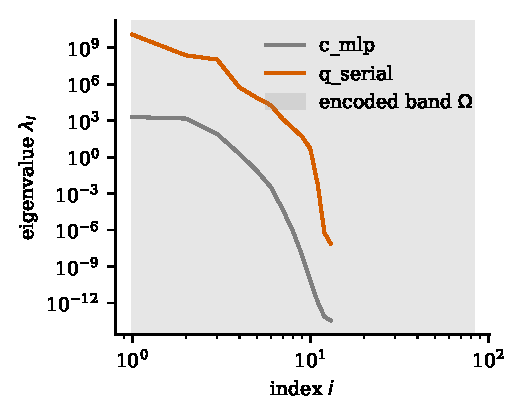
\includegraphics[width=0.48\linewidth]{figures/ntk_spectrum_poisson_pr7.pdf}\hfill
  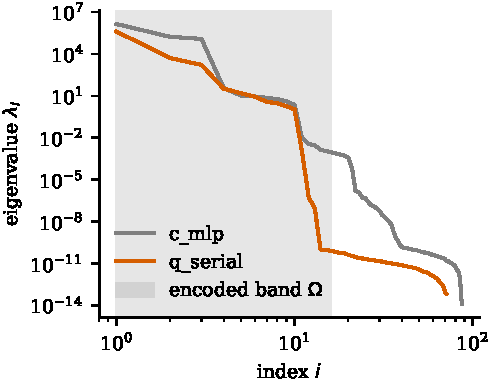
\includegraphics[width=0.48\linewidth]{figures/ntk_spectrum_helmholtz_k10_pr7.pdf}
  \caption{Residual NTK eigenvalue spectra at the final checkpoint, MLP
    (\texttt{c\_mlp}) against one copy of the SMCD circuit (\texttt{q\_serial}), seed 0,
    with the top-$|\Omega|$ index range shaded. Left:
    Poisson ($|\Omega|=81$ exceeds the circuit's 14 parameters). Right: Helmholtz
    $k{=}10$ ($|\Omega|=15$).}
  \label{fig:ntk}
\end{figure}

\subsection{Why one copy is not enough}
\label{sec:copyresult}

\paragraph{One copy learns the hard frequency and loses the easy one.} The Poisson
solution is $\sin\pi x+0.3\sin15\pi x$. Tracking the error at those two frequencies
(Figure~\ref{fig:specerr}), one copy cuts its $15\pi$ error to a median 10\% of its
starting value by step 1{,}000 (103\% for the Fourier-feature network, 86\% for the MLP,
51\% for the frequency-matched model). Its $\pi$ error falls to about 30\% by step
5{,}000 and then \emph{rises} to 1.9--2.0$\times$ its starting value by step 20{,}000, on
all five seeds, while the frequency-matched model reduces both. The residual loss weights
each Fourier mode of the error by $\omega^2$, so the $15\pi$ mode carries 225 times the
weight of the $\pi$ mode. A linear head on fixed sine features sets the two amplitudes
independently; a single circuit cannot, because all 81 of its amplitudes are functions of
the same ten angles read through one expectation value. Our reading, supported by these
data but not proven, is that the optimiser buys the heavily weighted amplitude at the
cost of the lightly weighted one. The loss agrees: it stalls near $3.3\times10^4$ from
step 1{,}000 while the error keeps moving, and the seeds agree closely (worst over best
$1.1\times$) because they converge to the same trade-off.

\begin{figure}[htbp]
  \centering
  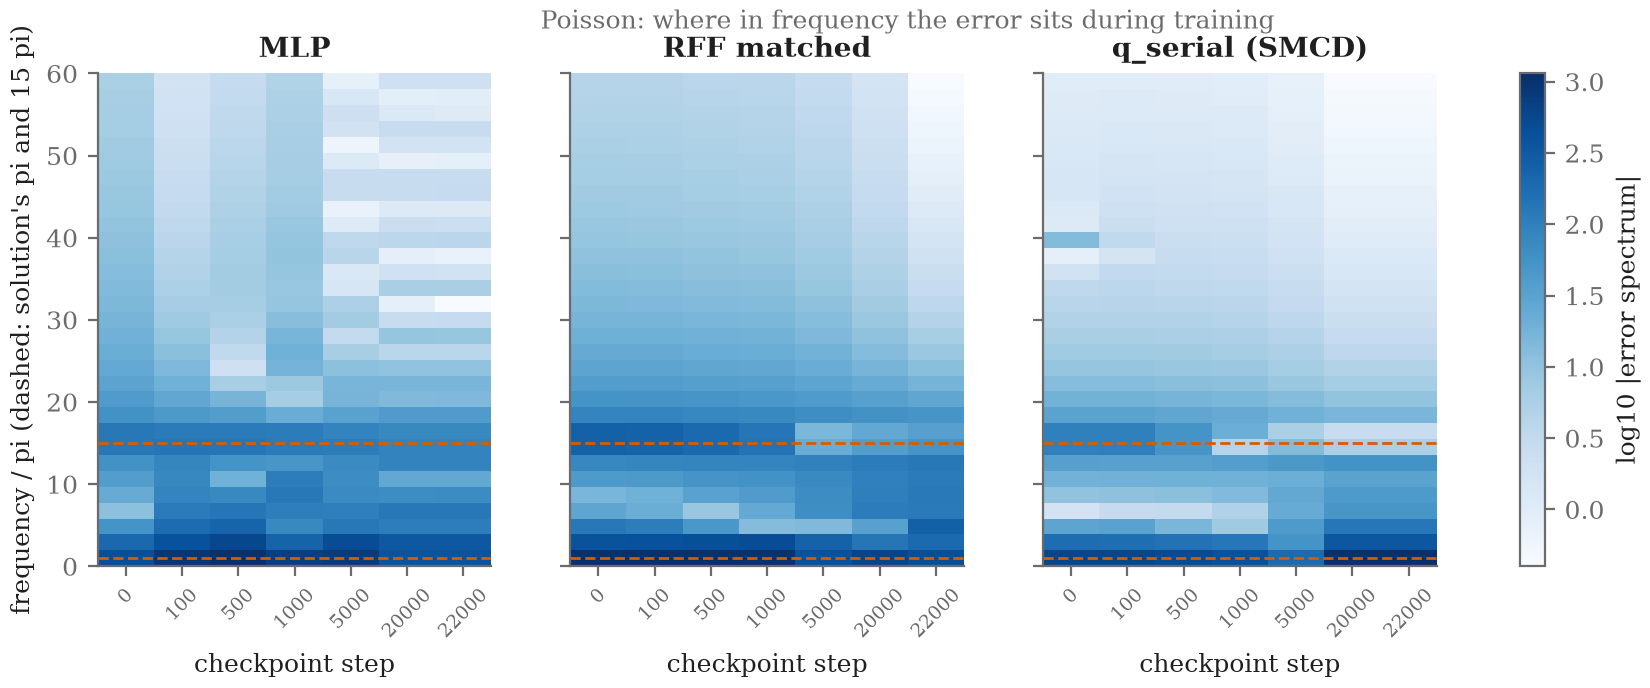
\includegraphics[width=\linewidth]{../results/report/figures/xai_spectral_error_poisson.png}
  \caption{Poisson, one copy: magnitude of the error spectrum at each checkpoint
    (seed 0), with the error at $\pi$ and $15\pi$ tracked over training.}
  \label{fig:specerr}
\end{figure}

\paragraph{Copies decouple the amplitudes.} Section~\ref{sec:copies}'s copies keep
$\Omega$ and give the head an independent handle on each copy. On the tuning seeds the
error falls with the number of copies, from 1.67 with one copy to 0.003 with eight at the
higher learning rate (Figure~\ref{fig:copies}); eight copies were selected.

\begin{figure}[htbp]
  \centering
  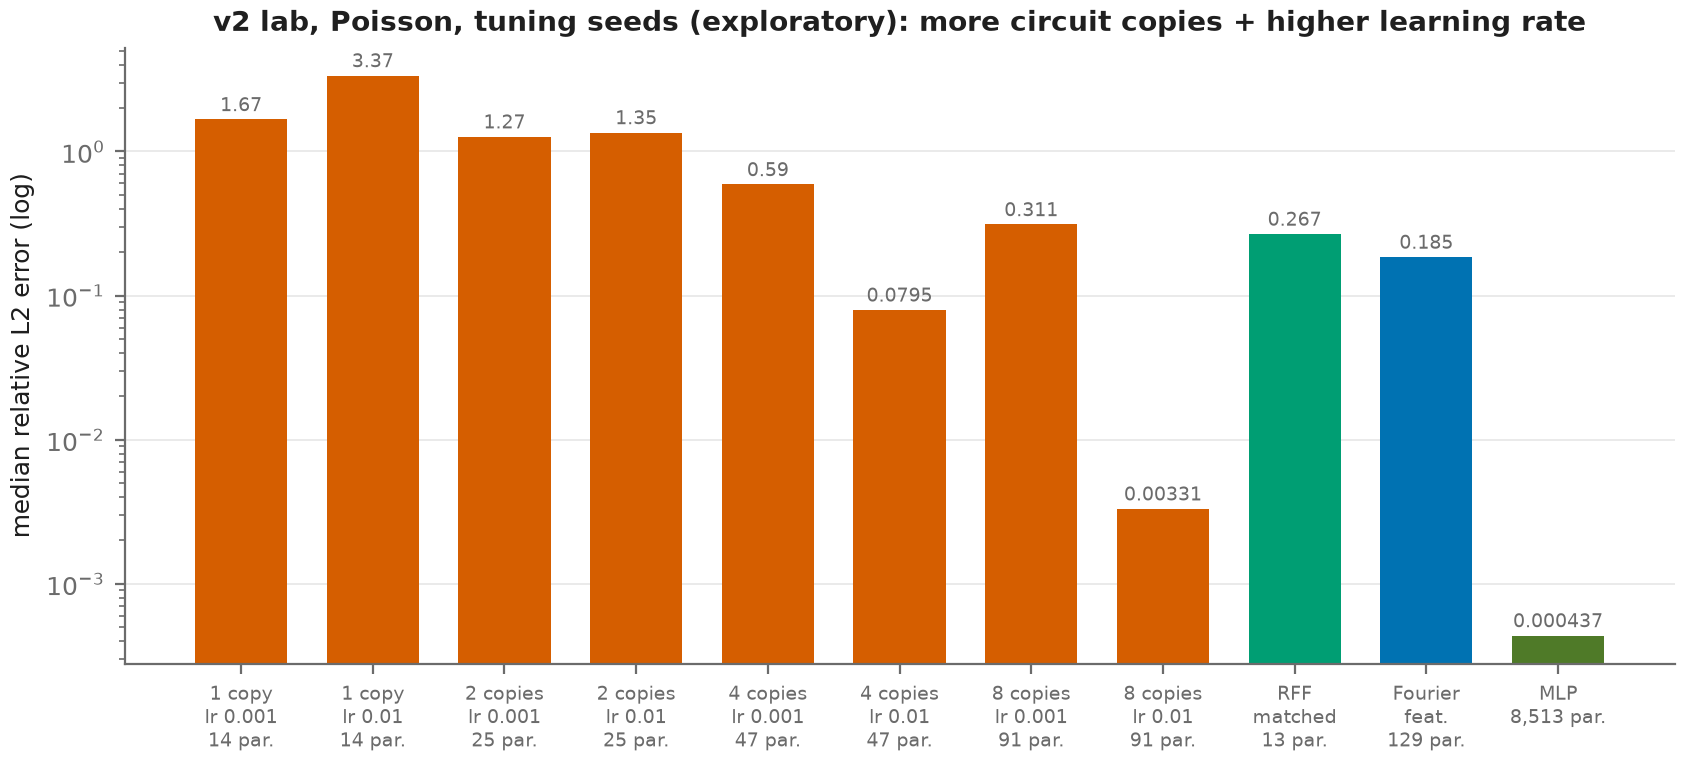
\includegraphics[width=\linewidth]{../results/report/figures/headline_v2_lab.png}
  \caption{Model selection on Poisson, tuning seeds 0--2: median error for 1, 2, 4 and 8
    copies at two learning rates, beside the best learning rate for each classical model.}
  \label{fig:copies}
\end{figure}

\paragraph{Eight copies on held-out seeds.} On seeds 10--14 (Table~\ref{tab:ensemble},
Figure~\ref{fig:ensemble}) the eight-copy circuit reaches a median error of 0.0037, with
every seed below 0.02. It beats the Fourier-feature network by three orders of magnitude
and the same circuit with random frequencies by $236\times$. The comparison with the MLP is
inconclusive: at its tuned learning rate the MLP failed on three of five seeds (1.2--3.6)
and reached 0.003--0.012 on the other two. The classical learning rates chosen on the
tuning seeds did not transfer well (the Fourier-feature network went from 0.19 to 5.0),
which inflates both of those ratios. \textbf{The frequency-matched classical model,
sized to the eight-copy circuit (83 parameters), is $3.3\times$ more accurate} (0.0011):
on Poisson, handing a classical model the frequencies SMCD reads off the equation works
better than the circuit.

% Generated by scripts/report/paper_tables.py from results/adjudication_v2.json.
\begin{table}[htbp]
  \centering
  \small
  \begin{tabular}{p{0.5\linewidth}lr}
  \toprule
  Claim & Verdict & Measured \\
  \midrule
  Beats the large MLP on Poisson ($\ge2\times$) & Inconclusive & 337.79$\times$ \\
  Beats Fourier features on Poisson ($\ge1.3\times$) & \textbf{Confirmed} & 1359.81$\times$ \\
  Matches the frequency-matched classical model on Poisson (within $1.3\times$) & Refuted & 3.30$\times$ \\
  Designed beats random frequencies, Poisson ($\ge1.5\times$) & \textbf{Confirmed} & 236.08$\times$ \\
  NTK flatter inside $\Omega$ than outside, Poisson & \textbf{Confirmed} & gap 15.2 \\
  Gain over the MLP lies inside $\Omega$, Poisson ($\ge70\%$) & \textbf{Confirmed} & 99.9\% \\
  Leaves the lazy-training regime earlier than classical models & Refuted & 2.53 vs 9.7e+04 \\
  Encoder drift stays below 0.2, so $\Omega$ stays valid & \textbf{Confirmed} & 0.10 \\
  \midrule
  Confirmed & 5 of 8 & \\
  \bottomrule
  \end{tabular}
  \caption{Pre-registered claims about the eight-copy SMCD circuit on Poisson, held-out seeds
    10--14. The baselines are sized to the eight-copy circuit where the claim names one.}
  \label{tab:ensemble}
\end{table}


\begin{figure}[htbp]
  \centering
  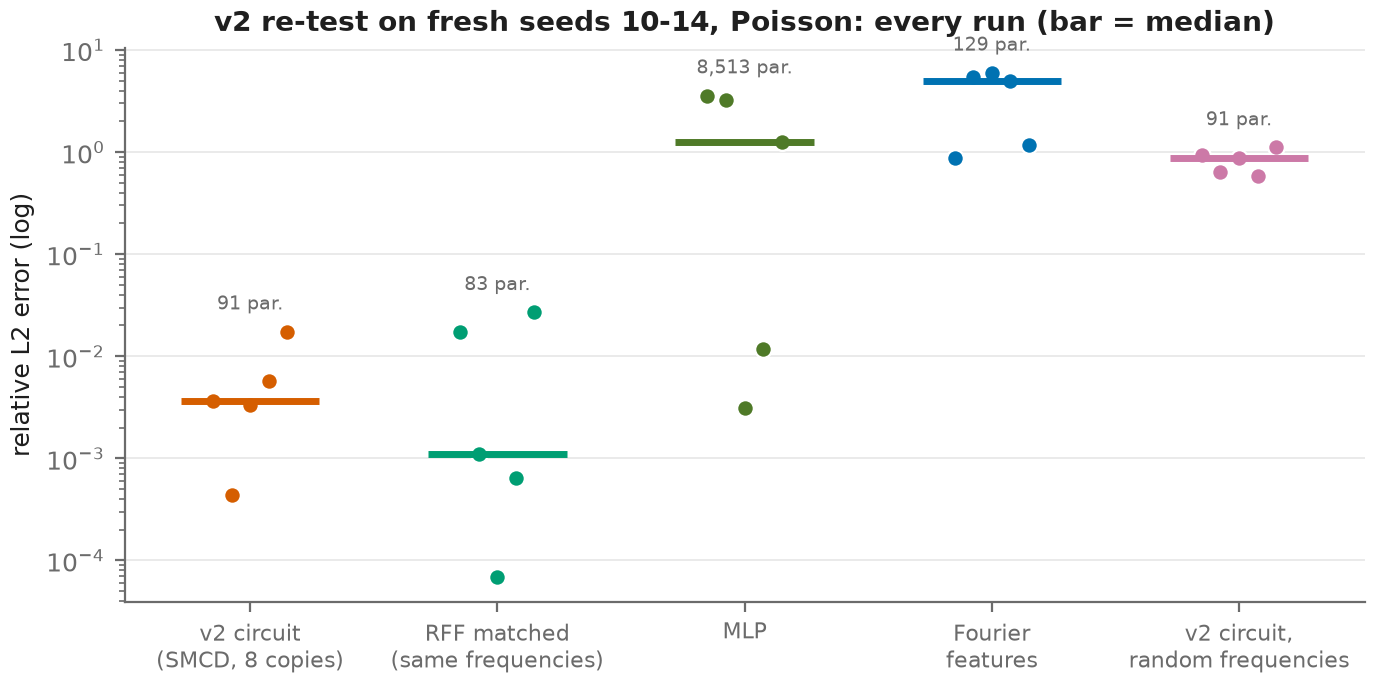
\includegraphics[width=0.9\linewidth]{../results/report/figures/headline_v2_retest.png}
  \caption{Poisson, held-out seeds 10--14: every run of the eight-copy circuit and the
    baselines (bar: median).}
  \label{fig:ensemble}
\end{figure}

\section{Negative Results}
\label{sec:negative}

\subsection{P2 (heat), C4's core claim: PR-4}
SMCD predicts near-zero benefit for a purely diffusive, smoothing operator
\emph{before any training run}, because $\sigma(k)$'s quadratic growth collapses the
target spectral support toward $k=0$ as $t$ increases (Section~\ref{sec:methodology},
Proposition~2): no family should beat \texttt{c\_mlp} by more than 5\% on P2. Measured
benefit, $(\text{median}_{\text{c\_mlp}}-\text{median}_{\text{family}})/
\text{median}_{\text{c\_mlp}}$, at $n=2$ seeds: \texttt{c\_ff} $+24.4\%$,
\texttt{c\_rff\_matched} $+34.9\%$, \texttt{q\_serial} $+7.7\%$, \texttt{q\_parallel}
$-67.5\%$, \texttt{q\_random} $-1023\%$, \texttt{q\_octave} $-51.2\%$.
\textbf{REFUTED} --- three families cross the 5\% bar. Two of the three violators
(\texttt{c\_ff}, \texttt{c\_rff\_matched}) are classical, so they bear on ``is \texttt{c\_mlp}
a strong baseline'' generically, not on SMCD's quantum-specific claim; \texttt{q\_serial}'s
$+7.7\%$ is the one genuine, if modest, violation of ``hybridization is harmless-at-best
on a smoothing operator.'' The other three quantum families do the opposite:
\texttt{q\_random} in particular is an order of magnitude \emph{worse} than \texttt{c\_mlp}
($-1023\%$), consistent with the mechanistic story (a high-frequency-rich, unmatched
circuit adding parameters and barren-plateau risk with nothing for the smoothing operator
to reward) --- just not uniformly true of every quantum family tested, which the 5\%
uniform bar could not distinguish and this per-family breakdown does.

\subsection{Negative-result map across all six instances}
\texttt{decision\_map} (\S\ref{sec:results}) plots SMCD's a-priori predicted benefit
against the measured \texttt{q\_serial}-vs-\texttt{c\_mlp} benefit, one point per
problem. Combined with \S\ref{sec:results}'s ablation (PR-1/PR-2/PR-3), the honest
summary at this sample size is that \texttt{q\_serial} underperforms every classical
family checked on P1 (Poisson) and does not clear its own falsifier against
\texttt{q\_random} on either P1 or P2 (PR-6, both INCONCLUSIVE at $n=2$) --- the
constructive C1 claim (spectrum-matched beats size-matched-random) has no confirming
evidence at the sample size this deadline allowed, not because the ratios point the
wrong way (PR-6/heat's $12.2\times$ ratio in the predicted direction) but because $n=2$
cannot statistically separate it from chance (see \S\ref{sec:results}'s sample-size
note).

\subsection{An unpredicted reversal: NTK drift (PR-11)}
Predicted: hybrid models leave the lazy/NTK-linear training regime earlier than
classical ones (larger $\|\Theta_t-\Theta_0\|/\|\Theta_0\|$ at 5k steps). Measured:
median hybrid drift $=1.03$, median classical drift $=6{,}878{,}097$ ($n=2$ each).
\textbf{REFUTED}, and not by a small margin --- classical models' NTK moved roughly
six-and-a-half million times further from initialization than hybrid models' did.
This is the sharpest reversal in the whole adjudication table and worth reading as a
finding in its own right, not just a failed prediction: at this checkpoint, on this
sample, it is the \emph{classical} parameters that are decisively non-lazy, while the
hybrid model's combined (classical + quantum) NTK stayed comparatively close to its
initialization. This is consistent with, though does not on its own establish, the
small-angle quantum initialization ($\sigma_0=0.1$, Section~\ref{sec:methodology})
constraining the hybrid model's effective learning dynamics near its NTK-linear regime
for longer than an unconstrained classical network's.

\subsection{Encoder drift stayed small (PR-12) --- the one clean methodological validation}
\textbf{CONFIRMED}: median $\|A-I\|_F=0.132$ at the final checkpoint, under the $0.2$
bar, $n=2$ runs. The encoder does not move far enough during training to invalidate the
$\Omega$/coverage claims computed once, at initialization (D3) --- the one prediction in
this table that both confirms cleanly and underwrites the validity of every other
frequency-domain claim in this paper (PR-7, PR-8, PR-9) as still describing the
\emph{trained} model, not just its untrained starting point.

\section{Limitations}
\label{sec:limitations}

\begin{enumerate}
\item \textbf{Simulation only, small circuits.} Every circuit runs on a statevector
  simulator; nothing here ran on quantum hardware, and noise is modelled by analytic
  surrogates checked against a density-matrix simulation. On the one-dimensional problems
  each circuit is one qubit without entanglement, which a classical computer evaluates
  cheaply, and simulation cost capped the experiments at 6--8 qubits. No claim of quantum
  computational advantage is made or tested.
\item \textbf{Where the method wins.} The eight-copy circuit's strongest result is one
  applied problem. On Poisson a classical model given the same frequencies remains
  $3.3\times$ more accurate, and at high Helmholtz wavenumbers no model learns the
  solution, so parity there says nothing about capability.
\item \textbf{Statistical power and baselines.} Five seeds give a smallest Wilcoxon $p$ of
  0.0625, so ``confirmed'' means all five seeds agree. In the six-problem matrix only the
  frequency-matched model and the random-frequency circuit are size-matched; the MLP and
  Fourier-feature network run at standard sizes. The eight-copy model was selected from a
  small grid of copy counts and learning rates, while classical families received a
  learning-rate search only.
\item \textbf{Design assumptions.} The encoder is restricted to an affine map so that
  $\Omega$ and coverage are well defined; achieved coverage does not by itself predict
  error; and the design card's predicted benefit is a heuristic, not a bound (it
  predicted 2.5\% on heat and zero on Helmholtz $k{=}4,10$, and the circuit beat the MLP
  on none of them).
\end{enumerate}

\section{Conclusion}
\label{sec:conclusion}

Spectrum-Matched Circuit Design turns the choice of a quantum circuit for a PDE into
arithmetic: the operator's Fourier symbol and the forcing give the frequencies the
solution needs, and the encoding scalings, depth, qubit count and entangler follow by
formula. The circuit it builds produces exactly the designed frequencies, and those
frequencies matter: against the same circuit with random ones, the designed circuit is
$6.5\times$ more accurate on the heat equation, $236\times$ on Poisson and $9.9\times$ on
groundwater, on every seed.

The explainability instruments showed what a single circuit cannot do. All of its
Fourier amplitudes depend on the same few angles, so on a solution that mixes a slow and
a fast wave the optimiser trades one for the other. Mixing eight copies of the designed
circuit through a linear head keeps the frequency set and frees the amplitudes. On
waterlogging of farmland from leaking canals, that model reaches 0.09\% error, $18\times$
more accurate than a classical network of the same size, and answers the planning
question to within 1\,m.

The results also mark the method's limits. On a smoothing operator no model beats a
plain MLP, as SMCD predicts before training; on Poisson a classical model handed the
same frequencies is $3.3\times$ more accurate than the circuit; and at high Helmholtz
wavenumbers every model fails. The most direct next steps are running the designed
circuits on quantum hardware, extending SMCD to problems of higher dimension, and
understanding when a trainable encoder lets the circuit beat fixed classical features at
the same frequencies, as it does on the groundwater problem.

\section{Post-submission errata (2026-09-25)}
\label{sec:errata}

Added after the WISER 2026 BQP Challenge; the version that was judged is repository tag
\texttt{v1.0-submission}. The pre-registered thresholds and all 15 verdicts are unchanged.
Every number below was re-derived from the committed runs; \texttt{FINDINGS.md} gives
the reproduction commands. E1--E3 are corrections, E4--E6 caveats the results understate.

\begin{description}
\item[E1 (PR-7).] The Helmholtz\_k10 decay-exponent gap is $-8.37$, not $-9.67$. The old
  value came from reloading gitignored checkpoints, before PR-7 was switched to the
  committed \texttt{xai/ntk\_step*.npz}. Still REFUTED.
\item[E2 (PR-8).] 99.9\%, not 71.3\%, of Poisson's improvement lies inside $\Omega$.
  Poisson's error spectrum is two-sided and $\Omega=-\Omega$, but the overlap code folded
  $\Omega$ onto $|\omega|$. So the mirrored half of the improvement (3{,}944 of 13{,}751
  units; 5{,}864 sit at $\omega=0$) counted as outside $\Omega$. Still CONFIRMED.
\item[E3 (figures).] The submitted heatmaps and \texttt{ntk\_spectrum\_p1/p4} shaded the
  design card's four encoding scalings ($\pi,3\pi,9\pi,27\pi$) as $\Omega$ instead of the
  realised frequency set (81 frequencies for Poisson). Adjudication always used the
  correct $\Omega$; the figures in this revision are regenerated.
\item[E4 (PR-9).] The coverage sweep trained at 1500+150 steps. Its six targets build
  only three distinct Poisson circuits: 0.4 and 0.6 give one, 0.8, 0.9 and 1.0 give
  another, and 0.2 gives a third. The 18 points are therefore 9 distinct measurements,
  and coverage is confounded with parameter count (8 vs.\ 14). At this budget full
  coverage wins on every seed (0.718--0.729 vs.\ 0.909--1.084). At the full 20000+2000
  budget the order reverses on two of three seeds: 1-layer circuits reach 0.66--0.70,
  while the 4-layer circuit stays at 1.54--1.58. Helmholtz\_k10 builds a single circuit
  at every target and scores 0.991--1.002 throughout.
\item[E5 (PR-3, PR-5).] At $k=10$ and $k=20$ every family's median rel-$L^2$ is
  0.977--1.089, while predicting $u\equiv0$ scores exactly 1. The CONFIRMED parity there
  is shared failure, not matched capability. SMCD's own predicted benefit is 0 at $k=4$
  and $k=10$.
\item[E6 (PR-1, PR-2).] The core matrix trained each family at its default size. On
  Poisson \texttt{q\_serial} has 14 parameters, \texttt{c\_mlp} 8{,}513 and
  \texttt{c\_ff} 129. Only \texttt{c\_rff\_matched} (13), \texttt{q\_random} (14) and
  \texttt{q\_octave} (13) are size-matched.
\end{description}

\section{Reproducibility appendix}
\label{sec:repro}

Every number below is measured against this session's actual runs, not estimated.

\begin{itemize}
\item \textbf{Hardware:} NVIDIA RTX 4090 Laptop GPU, 32 logical CPU cores
  (\texttt{provenance.json}, recorded per run) --- one machine for every run in this paper.
\item \textbf{Software} (\texttt{docs/ENV\_RESOLVED.md}, pinned via \texttt{uv}):
  Python 3.12.13, \texttt{torch 2.11.0+cu128} (CUDA 12.8), \texttt{pennylane 0.45.1},
  \texttt{numpy 2.4.4}, \texttt{scipy 1.18.0}.
\item \textbf{Determinism:} \texttt{qapinn.seeding.set\_global\_seed} seeds Python,
  NumPy, and Torch (CPU+CUDA) from one integer and enables
  \texttt{torch.use\_deterministic\_algorithms}; an explicit \texttt{torch.Generator}
  is threaded through every sampling call, so two runs at the same seed on the same device
  produce bit-identical \texttt{metrics.json} (T0.20). A CPU run and a CUDA run of the same
  configuration round differently (by $10^{-15}$ in rel-$L^2$ on a smoke run we re-checked;
  training can amplify such differences), and the run ID does not include the device.
\item \textbf{Seeds used} (state explicitly, cut from a pre-registered $n=5$ under the
  Aug 7 deadline --- Section~\ref{sec:limitations}, \texttt{FINDINGS.md} F10):
  \texttt{core\_matrix} $\{0,1\}$; \texttt{coverage\_sweep}/\texttt{alpha\_sweep}/
  \texttt{noise\_study}/\texttt{soft\_bc\_ntk} $\{0,1,2\}$; \texttt{depth\_sweep} $\{0\}$.
\item \textbf{Concurrency:} \texttt{--workers 2 --mem-fraction 0.35} for every sweep
  except \texttt{depth\_sweep} (\texttt{--workers 1 --mem-fraction 0.8}, forced down
  after system-memory exhaustion on its larger circuits --- OS/driver contention under
  concurrent CUDA context creation on this specific machine, not a VRAM limit).
\item \textbf{Measured wall-clock:} \texttt{tasks.py repro-quick} (CPU-only, 42
  combinations, implemented this session): \textbf{513.7\,s ($\approx$8.6 min)}, 42/42
  OK, under the 15-min target. \texttt{tasks.py test} (385 tests, post-submission
  revision): 244\,s CPU-only. \texttt{tasks.py figures} (20 figures from committed data, no GPU,
  byte-identical on the same machine): about 30\,s. \texttt{tasks.py repro-all} (added after submission):
  re-derives every figure and verdict from the committed runs in 56\,s; retraining all
  197 runs from scratch is 67.2\,h of training wall-clock on this machine (the sum of
  the runs' recorded \texttt{wall\_clock\_s}; \texttt{core\_matrix} alone is 58.5\,h).
\end{itemize}


\bibliographystyle{plainnat}
\bibliography{refs}

\end{document}
